\chapter{Introduction}

    L'innovation en matière de vision par ordinateur et d'intelligence artificielle ne cesse de progresser, souvent à des vitesses impressionnantes. Cette tendance ouvre de nouvelles perspectives passionnantes dans divers domaines, notamment celui de la capture de mouvement. C'est dans ce contexte que s'inscrit ce stage TN09 que j'ai eu l'opportunité de réaliser au sein de l'équipe BioMov-E du laboratoire BMBI (BioMécanique et BioIngénieurie) de l'UTC. Hier encore, les solutions en matières de motion capture reposaient principalement sur des systèmes utilisant des marqueurs physiques attachés au corps des sujets. Mais avec l'émergence de nouvelles technologies de vision par ordinateur et surtout d'intelligence artificielle, les solutions \textbf{markerless} deviennent de plus en plus crédible. Développer et mesurer la fiabilité de telles solutions est l'objectif principal de ce stage.

\section{Présentation du labo BMBI}
    \begin{figure}[h]
        \centering
        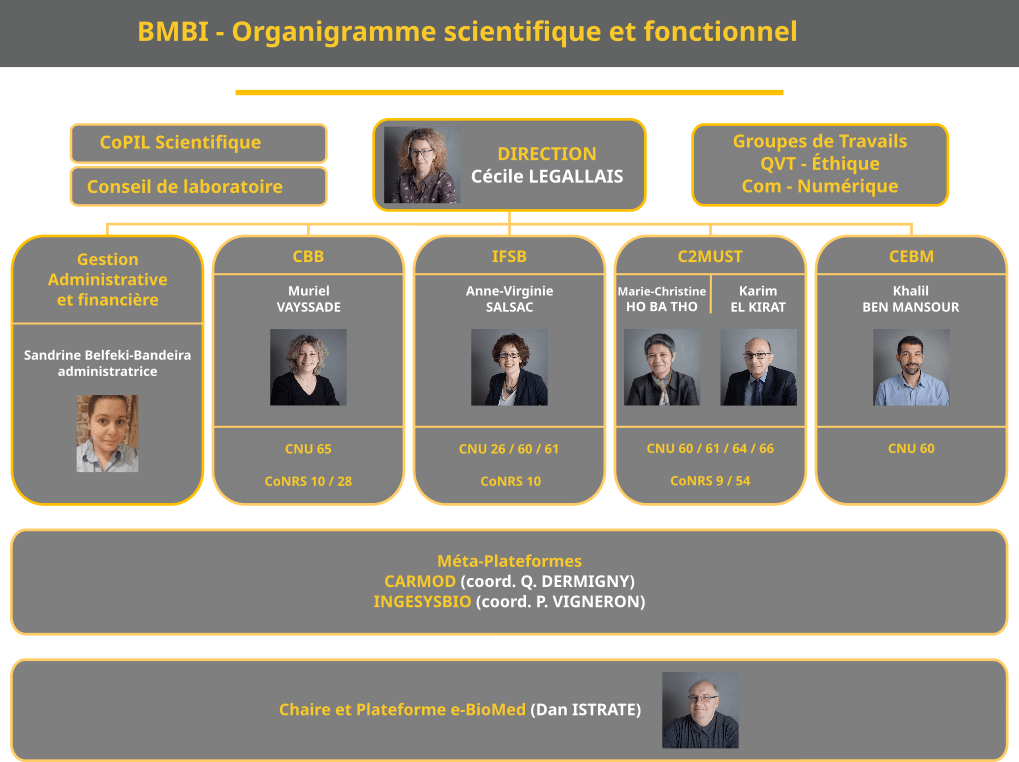
\includegraphics[width=0.6\textwidth]{assets/organigramme-fonctionnel-juillet2025.png}
        \caption{Organigramme du BMBI – \textit{bmbi.utc.fr/annuaire/}}
        \label{fig:organigramme-bmbi}
    \end{figure}

    Le laboratoire BMBI de l'UTC est un centre de recherche qui se concentre sur l'étude de la biomécanique et de la bio-ingénierie, et plus particulièrement sur la mécanique du vivant et l'ingénierie pour la santé. Associé au CNRS depuis 1982, il regroupe depuis plus de 40 ans plusieurs
    disciplines scientifiques telles que la mécanique, la biologie, l'électronique, le traitement du signal, l'informatique, la physique et la biochimie. En tout, il existe plus de 650 documents publiés dans des articles/revues scientifiques, et quasiment 100 thèses soutenues. Il est structuré en plusieurs équipes : Cellules Biomatériaux Bioréacteurs (équipe CBB), Interaction Fluides Structures Biologiques (équipe IFSB), caractérisation et modélisation personnalisée du Système Musculo-Squelettique (équipe C2MUST), et enfin l'équipe BioMov-E (ex CEBM) dans lequel j'ai été affilié durant mon stage.

    L'axe scientifique BioMov-E est né de la fusion entre deux entités complémentaires du BMBI : le Centre d'Expertise de Biomécanique du Mouvement (CEBM) et la chaire EBioMed (Objets Biomédicaux Connectés). Sa thématique de recherche principale porte sur le développement de modèles et de solutions permettant de suivre et d'analyser l'état de santé de l'Homme et de l'animal, d'évaluer sa performance et de prévenir les accidents ou le développement de pathologies.
    
    L'équipe BioMov-E s'appuie sur la plateforme Technologie Sport Santé (TSS) située au centre d'Innovation de l'UTC, qui comprend de nombreux équipements de pointe dédiés à l'analyse du mouvement humain. Des systèmes comme la technologie optoélectronique Hautes Résolutions du Vicon T160 (système de capture de mouvement avec marqueurs), des ergomètres, des plateformes de force, ainsi que des systèmes de test d’effort physique comme le Cosmed K5 sont utilisés pour étudier la biomécanique du mouvement dans divers contextes, allant de la rééducation à la performance sportive.

    TSS est l'une des plateformes les plus complètes en Europe dans le domaine de l'analyse du mouvement humain et a déjà servi de support dans plusieurs projets européens. Elle participe aussi au parcours pédagogique des étudiants de l'UTC, en leur offrant la possibilité de réaliser des stages et des projets de recherche appliqués dans le domaine de la biomécanique du mouvement. 

\section{Présentation de l'équipe BioMov-E}

    Durant le stage, j'étais intégré à l'équipe BioMov-E. Dirigé par mon tuteur de stage M. BEN MANSOUR, j'ai été accompagné par trois autres chercheurs/doctorants : Théophile COCQUEREZ, Julie PROCOPE-MAMERT et Guillaume TOFFOLI. J'étais aussi en contact régulier avec les autres membres de l'équipe BioMov-E lors de réunions. Enfin une autre stagiaire, Yiyang HUANG, effectuait aussi son TN09 sur le projet MoCapIA. À quelques mètres, on a pu échanger sur nos avancées, les méthodes à suivre, les difficultés rencontrées. Son travail concernait plus la poursuite du développement de l'interface utilisateur de l'application MoCapIA, en intégrant les fonctionnalités que je développais. Nous disposions chacun d'un bureau disposé dans un open-space avec les autres membres de l'équipe. Chaque semaine, nous avions une réunion avec M. BEN MANSOUR pour discuter de nos avancements ainsi que des prochaines étapes à suivre, et chaque mois, une réunion avec l'ensemble de l'équipe BioMov-E pour faire le point sur les différents projets en cours et partager nos résultats/difficultés. Le reste du temps, nous étions en autonomie et vraiment libre dans la façon d'accomplir le travail demandé. La méthode appliquée nous a été expliquée en début de stage, sur la manière d'effectuer un travail de rechercher, valider ses choix. Chaque étape commençait par une recherche bibliographique approfondie, et après avoir discuté avec le tuteur des différentes options possibles, nous pouvions commencer le développement. Enfin chaque ajout devait être testé et validé rigoureusement avec les métriques adaptées.

\section{Contexte Scientifique}

    La capture du mouvement (mocap) est un processus en plusieurs étapes : son but est d'extraire les mouvements d'une personne ou d'un objet à partir de données brutes, généralement des vidéos. C'est utilisé dans de nombreux domaines, allant de l'animation 3D dans les films et les jeux vidéos, à l'analyse biomécanique dans le domaine médical et sportif. Pour ça, il faut créer un modèle numérique 3D du mouvement à partir de points caractéristiques. Cette technologie est très utile dans le domaine de la santé comme la rééducation. Elle peut aussi être convoitée pour améliorer ses performances sportives. Avec un modèle 3D recréant le mouvement parfait, la détection du mouvement de l'athlète pourrait lui permettre de se rapprocher du geste parfait. 
    
    Traditionnellement, cela se faisait en utilisant des systèmes de capture de mouvement basés sur des marqueurs physiques attachés au corps du sujet. Ces marqueurs sont suivis par plusieurs caméras haute vitesse pour enregistrer leurs positions dans l'espace 3D, comme le système Vicon T160. Il dispose d'environs 40 caméras opto-électroniques à haute vitesse (jusqu'à 300 images par secondes) capables de suivre avec une grande précision les marqueurs réfléchissants placés sur le corps du sujet.

    Mais ces systèmes présentent plusieurs inconvénients majeurs. Ils sont coûteux, nécessitent un équipement spécialisé et une installation complexe. De plus, le port de marqueurs peut être inconfortable pour les sujets et peut influencer leur mouvement naturel. Ces limitations empêchent une adoption plus large, et notamment dans les domaines de la santé et du sport (comme mentionné précédemment) malgré leur fiabilité de l'ordre du dixième de millimètres. La plateforme BioMov-E dispose d'un tel système, le Vicon T160, qui s'avéra très utile pour mesurer et valider la précision de notre système en cours de développement introduit dans la prochaine section.

    Face à ces défis, une nouvelle approche de capture de mouvement \textbf{sans marqueurs} (markerless) a émergé. Cette méthode, entraînée par les avancées en intelligence artificielle, fait l'objet de plusieurs recherches récentes. En 2019, une entreprise canadienne \textit{Theia Markerless} a développé une technologie de ce genre. Crée et validée par des chercheurs, cette solution haut de gamme est certes précise, mais se rapproche finalement du coût et de la complexité des systèmes avec marqueurs (licence et matériels coûteux). D'autres équipes de recherches travaillent sur cette technologie, comme l'équipe CAMERA (Centre for the Analysis of Motion, Entertainment Research and Applications) de l'université de Bath au Royaume-Uni \cite{BATHResearch}. En partenariat avec l'Association de Bobsleigh britannique, l'équipe met au point un système de capture de mouvement markerless à l'aide de neuf caméras. Leurs objectifs sont comparables aux nôtres (voir section suivante).

    
\section{Objectif du stage}

    Notre but va donc être de développer un système de capture de mouvement \textbf{sans marqueurs} (markerless) en utilisant des techniques avancées de vision par ordinateur et d'intelligence artificielle. Ces techniques permettent de ne plus avoir besoin de marqueurs physiques, remplacé par des marqueurs virtuels détectés automatiquement dans les images. Le reste du processus – calibration, triangulation, reconstruction 3D - reste similaire. Cette approche offre plusieurs avantages : elle est plus flexible, moins coûteuse et permet une capture de mouvement plus naturelle. Cependant, elle présente aussi des défis techniques importants, car remplacer les marqueurs physiques par des marqueurs virtuels implique de nouvelles contraintes et imprécisions.
    \begin{figure}[ht]
    \centering
    \begin{subfigure}{0.48\textwidth}
        \centering
        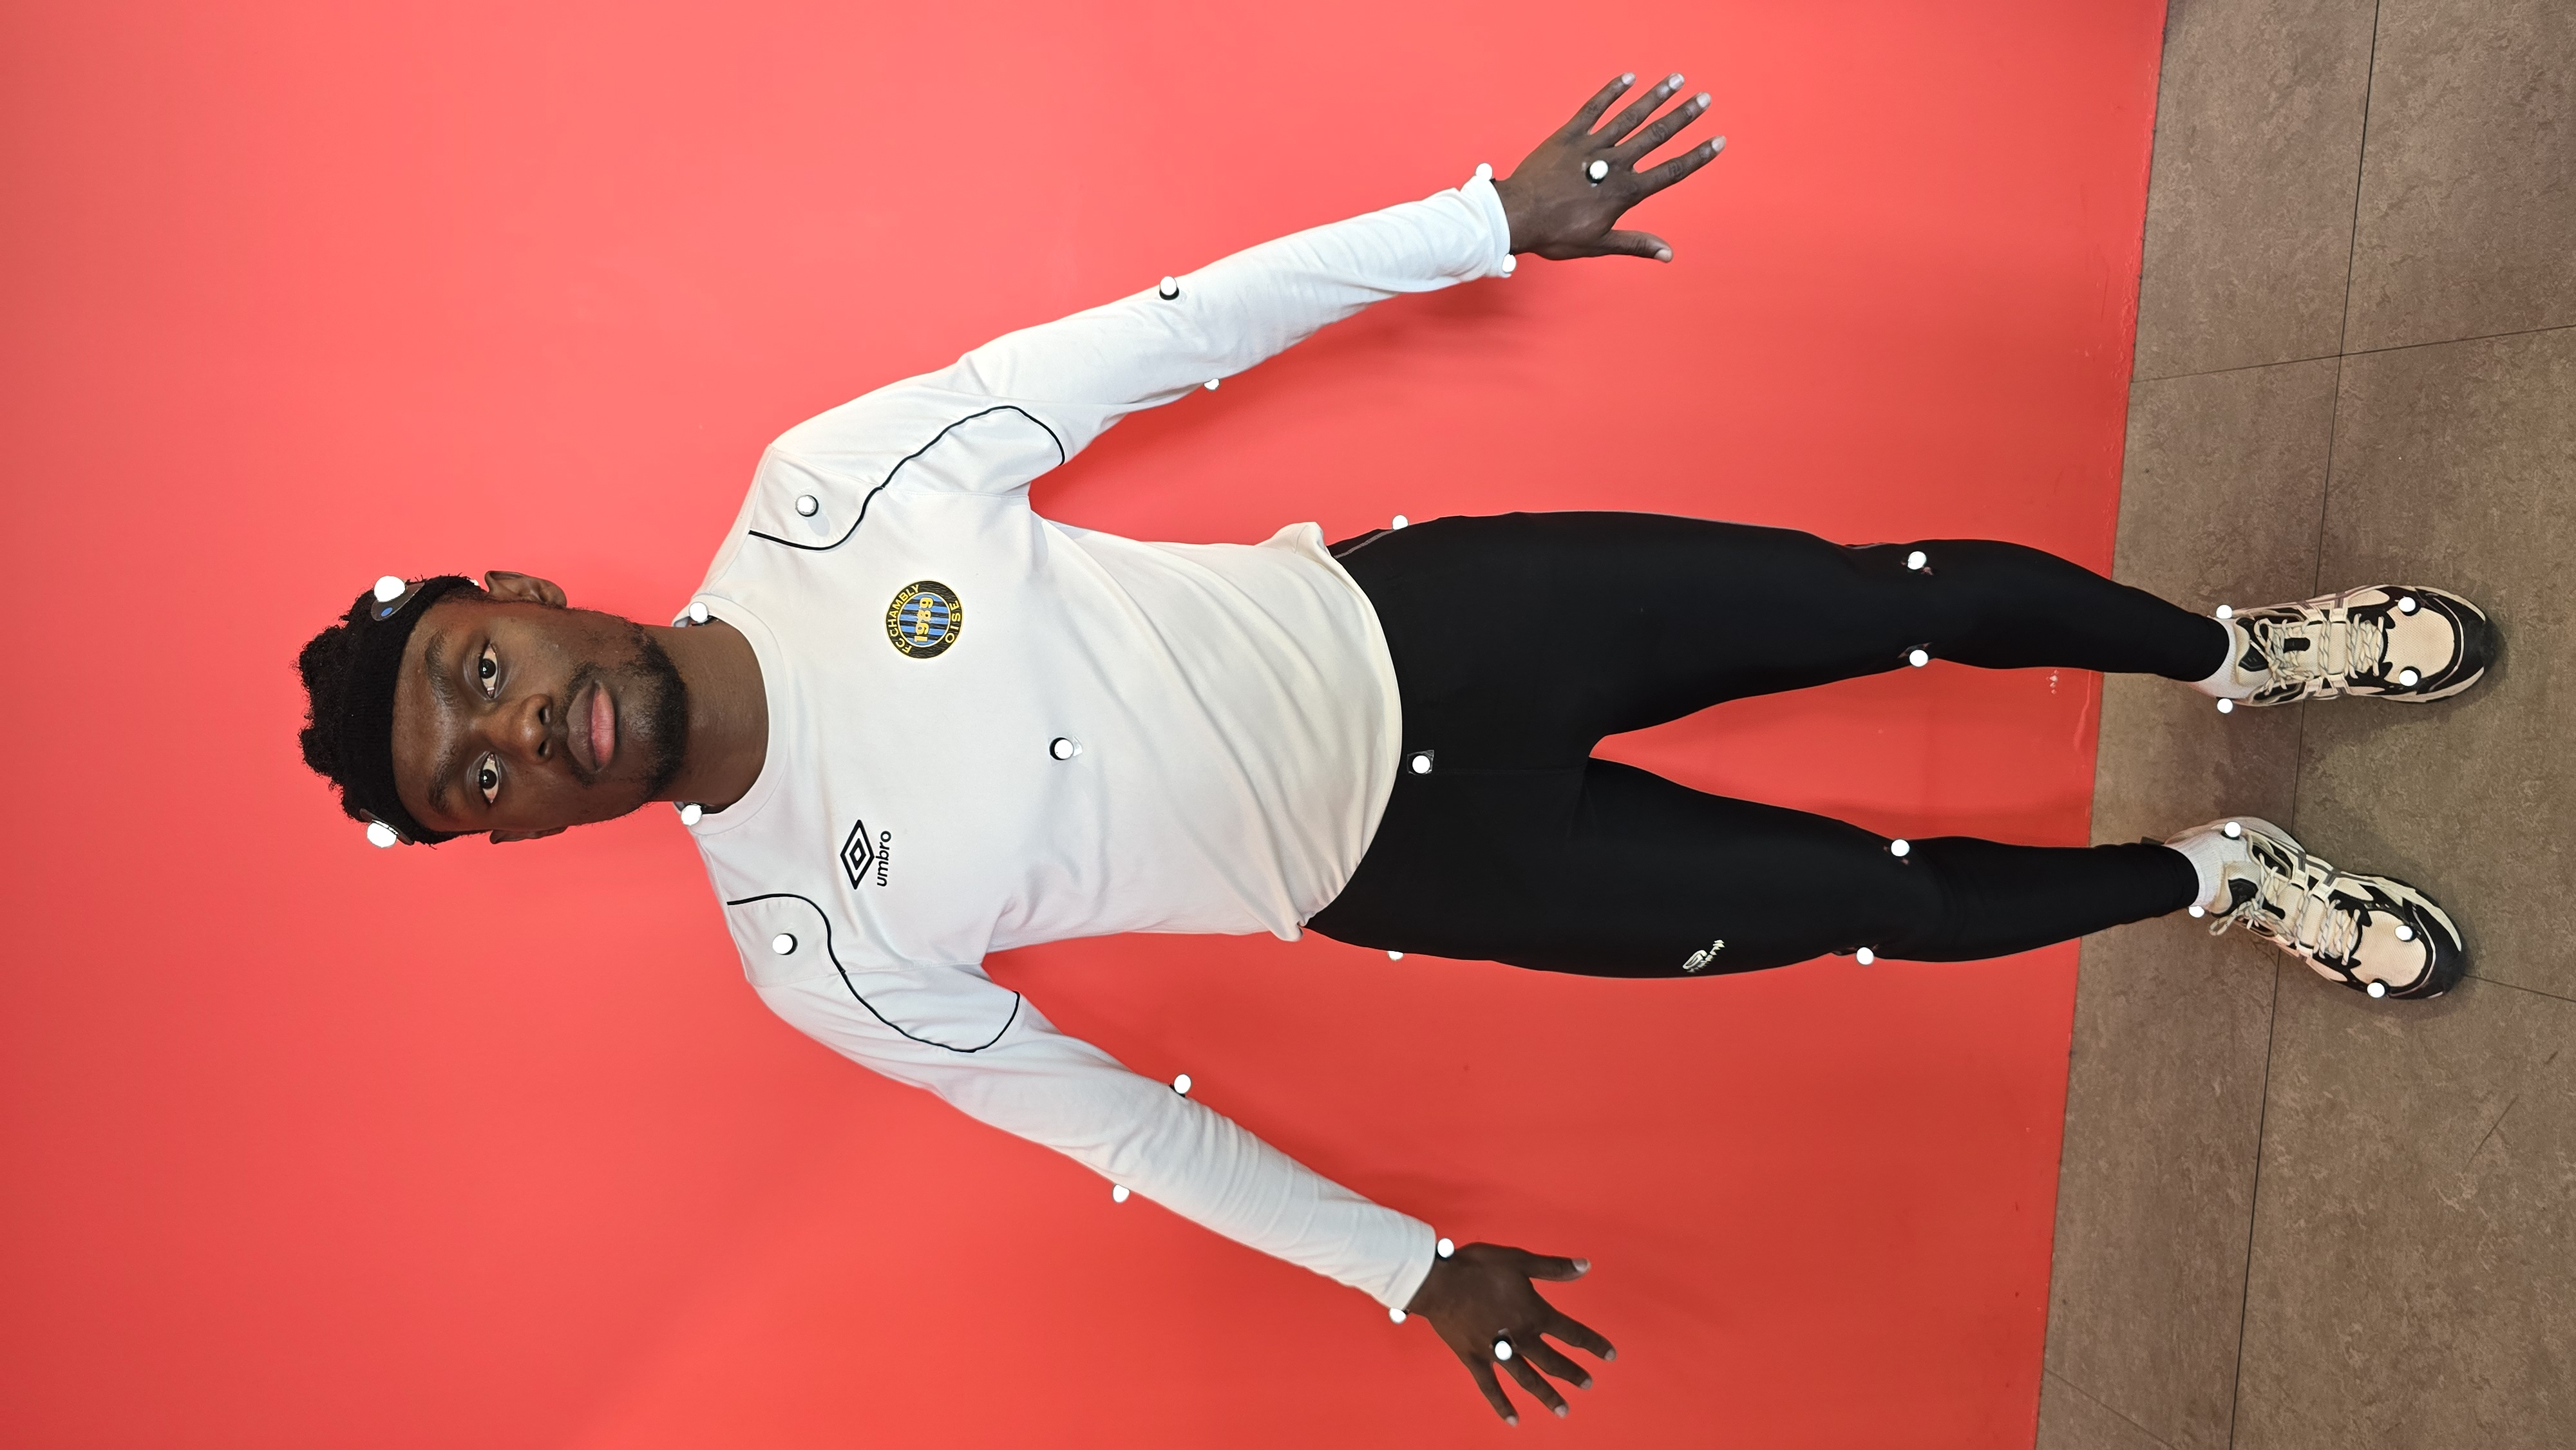
\includegraphics[width=\linewidth, angle=-90]{assets/Capture d'écran process/general/dorian_viconmarkers.jpg}
        \caption{Avec marqueurs}
        \label{fig:vicon-markers}
    \end{subfigure}% <--- Le signe % ici annule l'espace invisible
    \hfill
    \begin{subfigure}{0.48\textwidth}
        \centering
        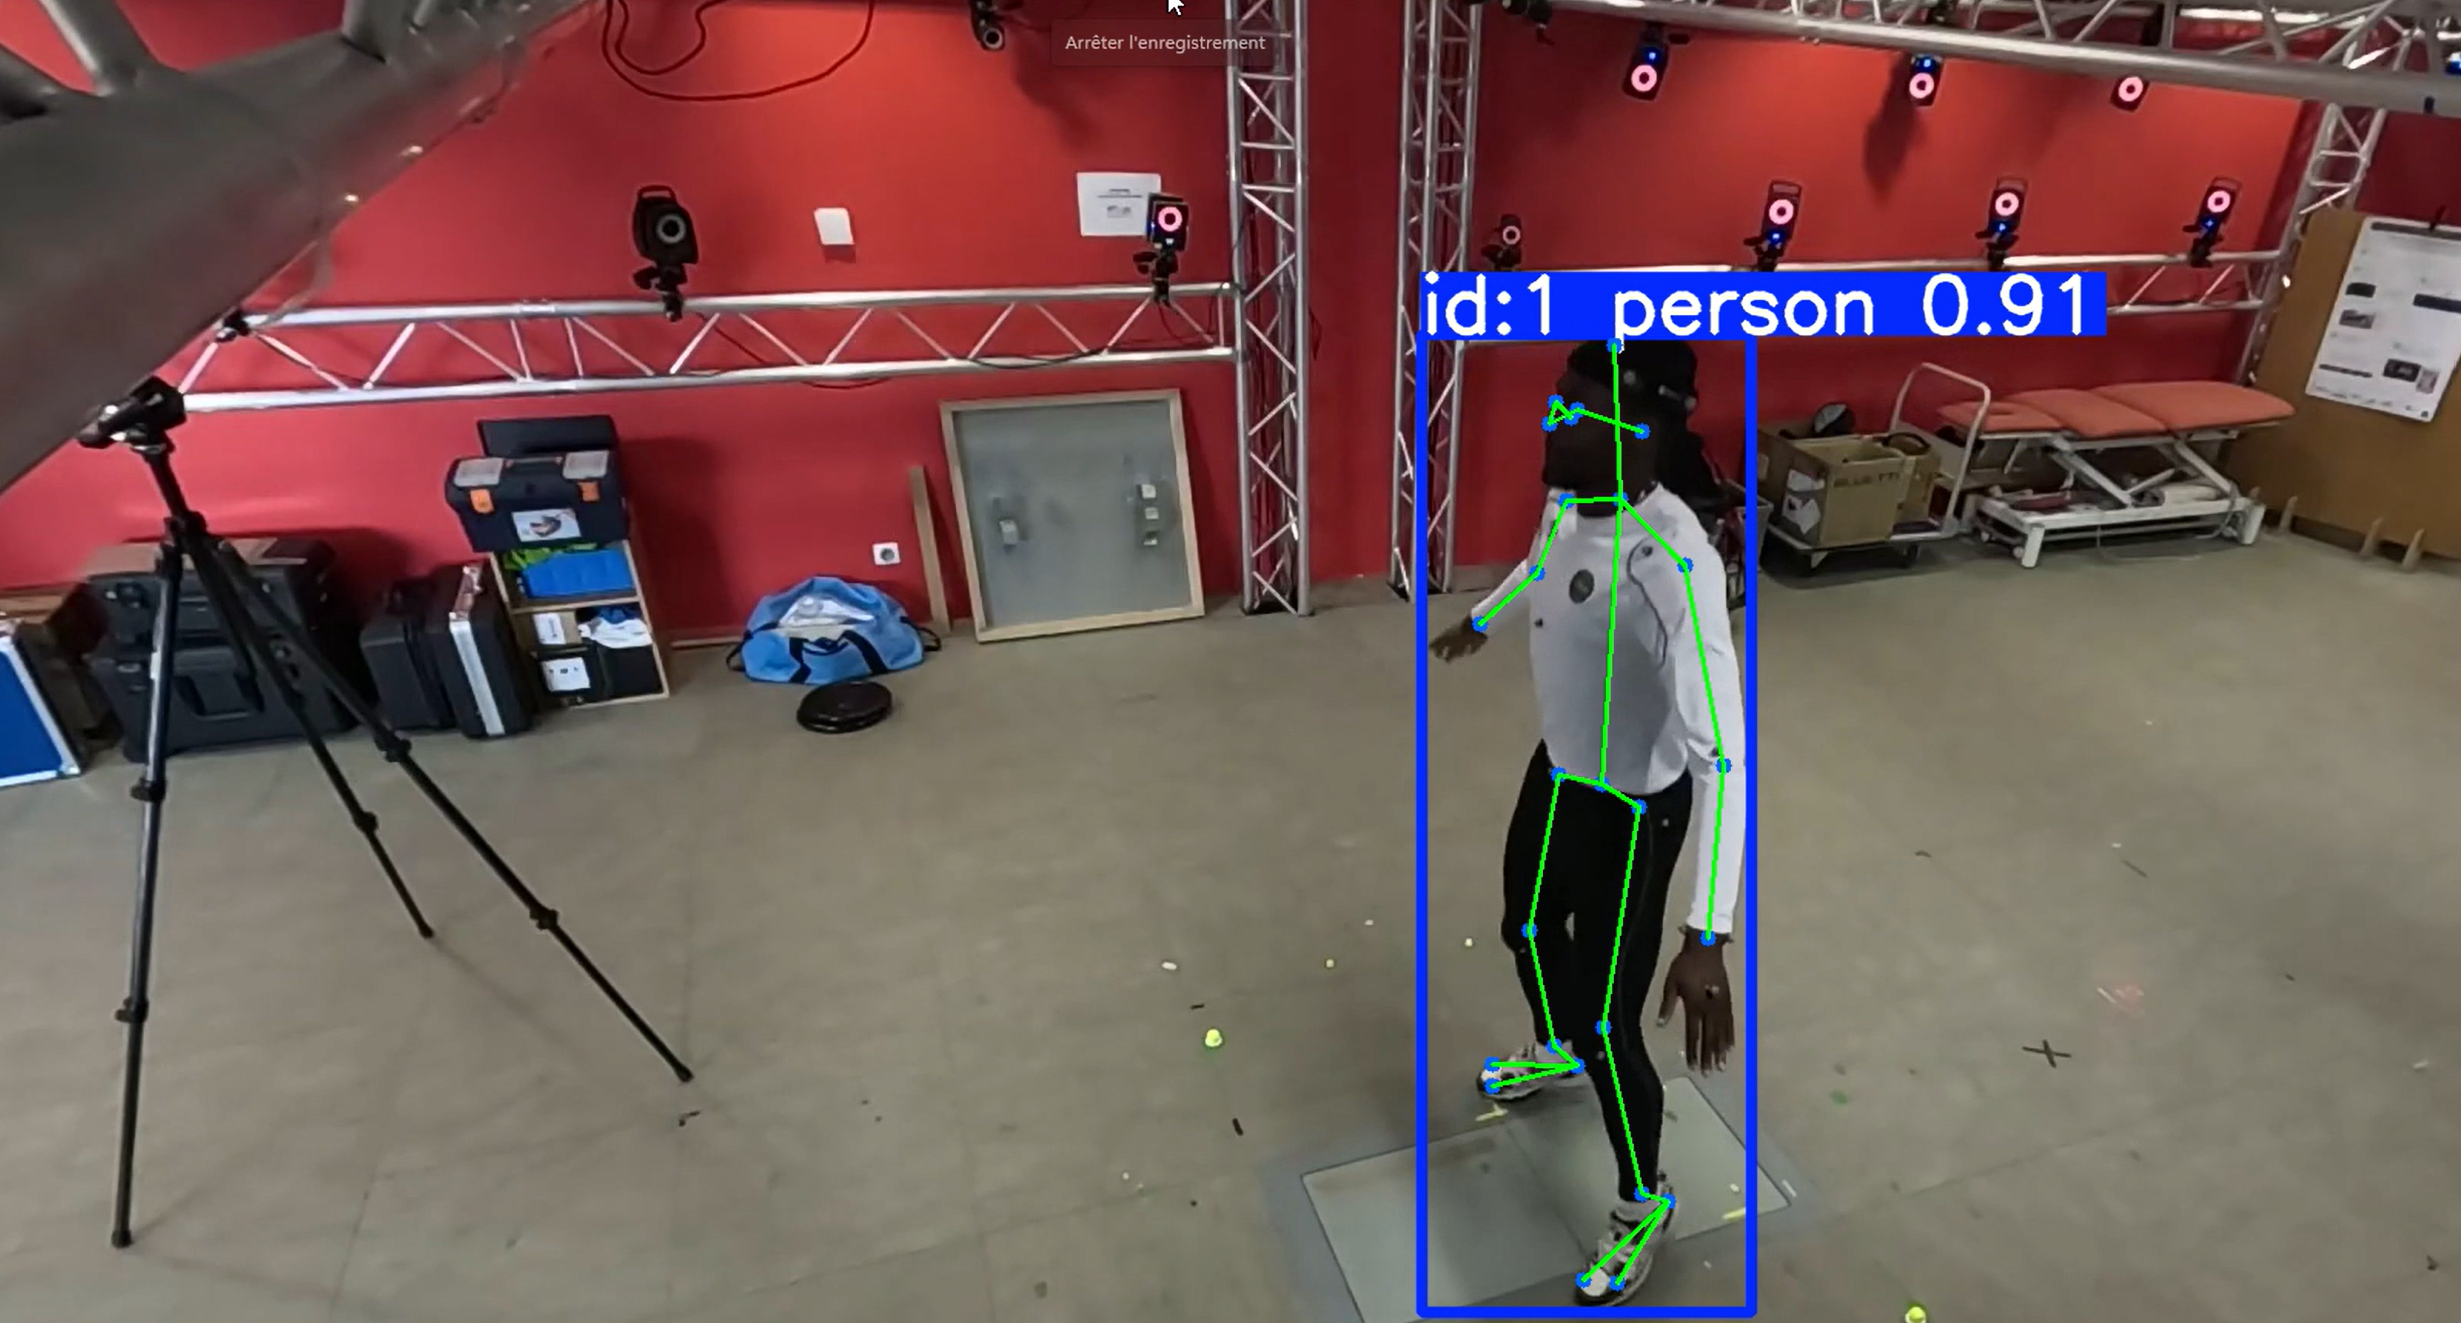
\includegraphics[width=\linewidth]{assets/Capture d'écran process/general/dorian_mocapmarker.png}
        \caption{Sans marqueurs}
        \label{fig:mocap-markers}
    \end{subfigure}
    \caption{Comparaison entre les systèmes de capture de mouvement avec et sans marqueurs}
    \label{fig:mocap-comparaison}
\end{figure}
    
    Durant les quatre derniers semestres, quatre stagiaires ont déjà effectué leur stage dans le cadre de ce projet. Les fonctions de bases ont été instaurées dès les premiers stagiaires comme la calibration, la synchronisation, la triangulation ainsi qu'un Ui (User Interface). L'ajout de fonctionnalités plus avancées autour de l'Ui a été instauré par le dernier stagiaire. L'objectif principal de mon stage est d'identifier la provenance des erreurs restantes afin d'améliorer la robustesse et la précision de la reconstruction 3D. Le but est de se rapprocher d'une précision et d'une capacité d'analyse biomécanique comparable à celle des systèmes avec marqueurs physiques comme le Vicon T160 et permettre l'utilisation en milieu clinique ou sportif.

    Dans le cadre d'un stage en \textbf{recherche}, il est aussi crucial de prendre en compte l'étendue de la littérature scientifique existante sur le sujet afin d'identifier de nouvelles approches et d'améliorer le système en général. Ce type de stage implique aussi une part importante de justification scientifique des choix techniques appliqués ou même rejetés.





\section{Déroulement du stage}
    Le stage s'est déroulé sur une période de 6 mois, de septembre 2025 à février 2026 avec deux semaines de fermeture du laboratoire durant les fêtes de fin d'année (du 20 décembre au 2 janvier).

    Même si le travail de programmation a représenté une part importante du stage, beaucoup de recherche et phases de test ont permis de rendre ce stage enrichissant dans plusieurs domaines. La compréhension du côté mathématique du processus a été aussi vraiment important pour pouvoir espérer améliorer la précision du système.

    Durant les deux premières semaines, il a fallu s'imprégner du contexte scientifique et technique du projet. Accompagné par le précédent stagiaire, on a d'abord, avec ma collègue, pris en main l'interface utilisateur qui permettait de gérer les différentes étapes de la capture de mouvement. On a pris connaissance aussi du "hardware" nécessaire pour le processus de capture, notamment les caméras, leur application, les différents damiers de calibration. En une semaine, on a pu maîtriser l'ensemble du processus, de l'acquisition des vidéos jusqu'aux données 3D et leur reconstruction dans l'espace. Ensuite, il a fallu consulter les anciens rapports, documents techniques et les articles scientifiques dans le domaine pour saisir l'ensemble des enjeux et défis du projet. En deux semaines, les fonctions principales du code ont été comprises, et des pistes d'amélioration ont été identifiées.

    Par la suite, une grosse période a été accordée à la recherche bibliographique. Cela s'est avéré être très utile surtout pour l'aspect mathématique, et m'as permis de mieux comprendre le fonctionnement interne de chaque étape et d'identifier les pistes d'améliorations.